\documentclass[letterpaper, 12pt]{article}
\usepackage{amsmath, amssymb}
\usepackage{mathtools}
\usepackage{graphicx}
\graphicspath{{./images/}}

\newtheorem{theorem}{Theorem}[section]
\newtheorem{lemma}[theorem]{Lemma}
\newtheorem{proposition}[theorem]{Proposition}
\newtheorem{corollary}[theorem]{Corollary}

\newenvironment{proof}[1][Proof]{\begin{trivlist}
\item[\hskip \labelsep {\bfseries #1}]}{\end{trivlist}}
\newenvironment{definition}[1][Definition]{\begin{trivlist}
\item[\hskip \labelsep {\bfseries #1}]}{\end{trivlist}}
\newenvironment{example}[1][Example]{\begin{trivlist}
\item[\hskip \labelsep {\bfseries #1}]}{\end{trivlist}}
\newenvironment{remark}[1][Remark]{\begin{trivlist}
\item[\hskip \labelsep {\bfseries #1}]}{\end{trivlist}}

\newcommand{\qed}{\quad \blacksquare}
\newcommand{\keyword}[1]{\textbf{#1}}
\newcommand{\then}{\rightarrow}
\newcommand{\bithen}{\leftrightarrow}
\DeclareMathOperator{\lcm}{lcm}
\DeclareMathOperator{\Dom}{Dom}

\newcommand{\N}{\mathbb{N}}
\newcommand{\Z}{\mathbb{Z}}
\newcommand{\Q}{\mathbb{Q}}
\newcommand{\R}{\mathbb{R}}
\newcommand{\C}{\mathbb{C}}
\newcommand{\0}{\emptyset}
\newcommand{\power}{\mathcal{P}}

\newcommand{\divby}{\; \vdots \;}

\title{MATH 381 HW 7 part 4}
\author{Christian Jahnel}
\date{27 April 2024}

\begin{document}
\maketitle
\begin{enumerate}
\item Let $f: \R^2 \to \R$ be given by $f(x, y) = x - y$. Determine, with proofs, whether $f$ 
is one-to-one, onto, both, or neither. Be sure to fully justify both your statement of 
one-to-one and your statement of onto.
\begin{enumerate}
\item $P: \text{$f$ is an injective (i.e. one-to-one) function}$
\[\begin{split}
    P &\equiv \forall (x_1, y_1), (x_2, y_2) \in \R^2(f(x_1, y_1) = f(x_2, y_2) 
    \then (x_1, y_1) = (x_2, y_2)) \\
    &\equiv \forall (x_1, y_1), (x_2, y_2) \in \R^2((x_1, y_1) \ne (x_2, y_2) 
    \then f(x_1, y_1) \ne f(x_2, y_2))
\end{split}\]
Suppose $(x_1, y_1) \ne (x_2, y_2)$ and let $x_1 = y_1$ and $x_2 = y_2$.
\begin{gather*}
\begin{aligned}
    f(x_1, y_1) = x_1 - y_1 = x_1 - x_1 = 0 \\
    f(x_2, y_2) = x_2 - y_2 = x_2 - x_2 = 0
\end{aligned}
\implies f(x_1, y_1) = f(x_2, y_2)
\end{gather*}
\[\begin{split}
    &\therefore \exists (x_1, y_1), (x_2, y_2) \in \R^2 ((x_1, y_1) \ne (x_2, y_2) 
    \then f(x_1, y_1) = f(x_2, y_2)) \\
    &\implies \neg P
\end{split}\]
\item $Q: \text{$f$ is a surjective (i.e. onto) function}$
\[Q \equiv \forall z \in \R \; \exists x, y \in \R^2(f(x, y) = z)\]
Let $z \in \R$.
\begin{align*}
    \text{Fix } y &= 0 \in \R \\
    \implies z = x - y &\iff z = x \\
    z \in \R &\implies x \in \R
\end{align*}
$\therefore Q \qed$
\end{enumerate}
\begin{flushleft}
    Consequently, \textbf{$f$ is a surjective (i.e. onto) function}, but \textbf{it is not an 
    injective (i.e. one-to-one) function}, and thus it cannot be a bijective function. 
    Intuitively, for every value $z$ on the $z$-axis of the 3-D graph of $f$, there must be a 
    one-dimensional (linear) slice through the plane. Consequently, there are an infinite amount 
    of solutions along each line, and therefore it cannot be injective. As for the surjective 
    property, the plane spans all real numbers in its range since it is angled nonparallel to 
    the $x$-axis, as seen by its coefficients.
\end{flushleft}
\item Suppose $f: A \to B$ is one-to-one and $g: B \to C$ is one-to-one. 
Prove $g \circ f: A \to C$ is also one-to-one.
\begin{multline*}
    \forall x_A, y_A \in A(f(x_A) = f(y_A) \then x_A = y_A) \\
    \wedge \forall x_B, y_B \in B(g(x_B) = g(y_B) \then x_B = y_B)
\end{multline*}
\[P: \forall x_A, y_A \in A((g \circ f)(x_A) = (g \circ f)(y_A) \then x_A = y_A)\]
Let $x_A, y_A \in A$ and suppose $(g \circ f)(x_A) = (g \circ f)(y_A)$.
\begin{align*}
    (g \circ f)(x_A) &= (g \circ f)(y_A) \\
    \implies g(f(x_A)) &= g(f(y_A))
\end{align*}
\begin{align*}
    \text{Let } x_B &= f(x_A) \in B \\
    \text{Let } y_B &= f(y_A) \in B
\end{align*}
\begin{align*}
    g(f(x_A)) &= g(f(y_A)) \\
    \implies g(x_B) &= g(y_B) \\
    \implies x_B &= y_B \\
    \implies f(x_A) &= f(y_A) \\
    \implies x_A = y_A
\end{align*}
$\therefore P \qed$
\pagebreak
\item Let $A = \{1,2,3,4,5\}$ and define relations $R$ and $S$ on $A$ by $R = \{(1,2),(2,2),(4,3)\}$ 
and $S = \{(2,1),(3,3),(3,5),(5,4)\}$. Determine the matrix for the relation $S \circ R$.
\begin{gather*}
    S := \begin{bmatrix}
        0 & 0 & 0 & 0 & 0 \\
        1 & 0 & 0 & 0 & 0 \\
        0 & 0 & 1 & 0 & 1 \\
        0 & 0 & 0 & 0 & 0 \\
        0 & 0 & 0 & 1 & 0
    \end{bmatrix} \qquad
    R := \begin{bmatrix}
        0 & 1 & 0 & 0 & 0 \\
        0 & 1 & 0 & 0 & 0 \\
        0 & 0 & 0 & 0 & 0 \\
        0 & 0 & 1 & 0 & 0 \\
        0 & 0 & 0 & 0 & 0
    \end{bmatrix} \\
    S \circ R := \begin{bmatrix}
        1 & 0 & 0 & 0 & 0 \\
        1 & 0 & 0 & 0 & 0 \\
        0 & 0 & 0 & 0 & 0 \\
        0 & 0 & 1 & 0 & 1 \\
        0 & 0 & 0 & 0 & 0
    \end{bmatrix}
\end{gather*}
\item Given the relation $R$ on $\{a,b,c,d\}$ defined by the digraph below, determine, with 
justification, whether $R$ is symmetric, transitive, and/or reflexive. Provide explanation for 
each of the three properties. \\
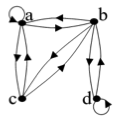
\includegraphics{digraph}
\begin{enumerate}
    \item The relation is \textbf{not reflexive} because only $a$ and $d$ point back to 
    themselves. $b$ and $c$ do not share this characteristic.
    \item The relation is \textbf{symmetric} because each element that is related to another 
    shares a relation from that element. In other words, each element is bidirectionally related 
    to its related elements.
    \item The relation is \textbf{not transitive} because related elements do not necessarily 
    share relations with the related elements' related elements. For example, $(a,b) \in R$ and 
    $(b, d) \in R$, however $(a, d) \notin R$.
\end{enumerate}
\pagebreak
\item Let $R$ be a relation on $\N$ that is symmetric and transitive. Further, suppose that 
$(x,7) \in R$ for all $x \in \N$. Show that $R$ induces a partition on $\N$.
\begin{align*}
    \intertext{Since $R$ is symmetric:}
    \forall x \in \N ((x,7) \in R) \then \forall x \in \N ((7, x) \in R) \\
    \intertext{Let $x, y \in \N \quad x \ne y$. Since $R$ is transitive:}
    (x, 7) \in \R \wedge (7, y) \in \R \then (x, y) \in \R
\end{align*}
Since $x, y$ are arbitrary positive integers, any two are related. 
Consequently, every element from $\N$ will be mapped to every element of $\N$. Therefore, every 
element in $\N$ is in the same subset which forms a partition over itself.
\item Let $S = \power(\{1,2,3,4,5\})$, the power set of the set of the first five positive 
integers. Define a relation $R$ on $S$ as follows: set $A$ is related to set $B$ via $R$ if and 
only if $|A|=|B|$.
\begin{enumerate}
\item Determine the equivalence class $[\{2,3\}]$.
\[[\{2,3\}] = \{\{1,2\},\{1,3\},\{1,4\},\{1,5\},\{2,3\},\{2,4\},\{2,5\},\{3,4\},\{3,5\},\{4,5\}\}\]
\item Determine the equivalence class $[\emptyset]$.
\[[\emptyset] = \{\emptyset\}\]
\item How many distinct equivalence classes does $R$ have? Explain your answer. \\
\\
$R$ has six distinct equivalence classes because the relation is dependent on the cardinality 
of subsets. Since a subset can have zero elements at minimum (this would be the empty 
set) and five elements at maximum (the set itself), the possible cardinalities of subsets are 
0,1,2,3,4,5. There are 6 possible cardinalities of subsets, so there should be \textbf{6} 
distinct equivalence classes.
\end{enumerate}
\end{enumerate}
\end{document}
